\documentclass[pdf]{beamer}
\mode<presentation>{}

\newcommand{\G}{\textcolor{blue}{G}}
\newcommand{\Gone}{\textcolor{blue}{G_1}}
\newcommand{\Gtwo}{\textcolor{blue}{G_2}}
\newcommand{\Gthree}{\textcolor{blue}{G_3}}
\newcommand{\n}{\textcolor{red}{n}}
\newcommand{\V}{\textcolor{teal}{V}}
\newcommand{\E}{\textcolor{olive}{E}}
\newcommand{\T}{\textcolor{orange}{T}}
\newcommand{\bluea}{\textcolor{blue}{a}}
\newcommand{\blueb}{\textcolor{blue}{b}}
\newcommand{\bluec}{\textcolor{blue}{c}}
\newcommand{\blued}{\textcolor{blue}{d}}
\newcommand{\bluee}{\textcolor{blue}{e}}
\newcommand{\bluef}{\textcolor{blue}{f}}
\newcommand{\blueg}{\textcolor{blue}{g}}
\newcommand{\ore}{\textcolor{gold}{\Omega}}
\newcommand{\orefirstcond}{\textcolor{gold}{\Omega_1}}
\newcommand{\oresecondcond}{\textcolor{gold}{\Omega_2}}
\newcommand{\gdeg}{\text{deg}}
\newcommand{\jump}{\hspace{10px}}
\definecolor{gold}{rgb}{0.85,0.65,0.13}

\setbeamertemplate{itemize items}[circle]

\usepackage{multicol,mathtools,cancel,slashed,xcolor,color,tikz}
\usefonttheme{serif}

%% preamble
\title{Ore's Theorem}
\subtitle{CS 111 Presentation}
\author{Youssef Adam \and Thomas Kang \\ Youssef Koreatam \and Michael Wong \and Gabriel Serrano}
\date{March 19, 2024}
\institute{Department of Computer Science, University of California, Riverside}
\begin{document}

    %% title frame
    \begin{frame}
        \titlepage
    \end{frame}

    %% questions
    \begin{frame}{Introduction: Questions}
        Below are three questions that you may be able to answer by the end of this presentation.
        \vspace{10px}
        \begin{itemize}
            \item What are the two criteria a graph must meet in order to satisfy Ore's theorem and therefore be a Hamiltonian graph?
            \item If a graph $\G$ does not meet both criteria to satisfy Ore's theorem, is $\G$ Hamiltonian?
            \item What is one example of a real-world application of Hamiltonian cycles, and how does this tie in with Ore's theorem?
        \end{itemize}
    \end{frame}

    %% introduction frame
    \begin{frame}{Introduction: Background Knowledge}
        To understand \textbf{Ore's theorem}, we must briefly recapitulate
        what it means for a graph to be \textbf{Hamiltonian}.
        \pause
        \vspace{10px}
        \\Let $\G(\V,\E)$ be an undirected graph with $|\V| \geq 3$ vertices. \pause
        \\If we are able to create a cycle $\T$ that meets each and every
        vertex strictly once, then $\G$ is considered \textbf{Hamiltonian}.
        \pause
        \vspace{20px}
        \\\textcolor{cyan}{\underline{Example:}}
        \vspace{10px}
        \begin{figure}
            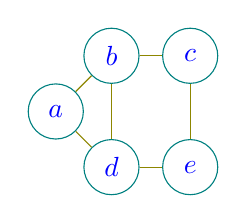
\begin{tikzpicture}[auto,node distance=1cm,scale=1, main/.style = {minimum size=0.7cm, color=teal, draw, circle},
                every path/.style = {color=olive}]
                \node[main] (1) {$\bluea$};
                \node[main] (2) [above right of=1] {$\blueb$};
                \node[main] (3) [right of=2] {$\bluec$};
                \node[main] (4) [below right of=1] {$\blued$};
                \node[main] (5) [right of=4] {$\bluee$};
                \path[every node/.style={font=\sffamily\small}]
                    (1) edge node [right] {} (2)
                    (1) edge node [right] {} (4)
                    (2) edge node [right] {} (4)
                    (2) edge node [right] {} (3)
                    (4) edge node [right] {} (5)
                    (3) edge node [right] {} (5);
            \end{tikzpicture}
            \pause
            \hspace{50px}
            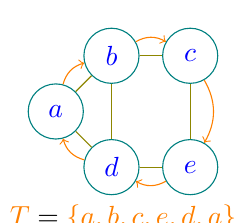
\begin{tikzpicture}[auto,node distance=1cm,scale=1, main/.style = {minimum size=0.7cm, color=teal, draw, circle}]
                \node[main] (1) {$\bluea$};
                \node[main] (2) [above right of=1] {$\blueb$};
                \node[main] (3) [right of=2] {$\bluec$};
                \node[main] (4) [below right of=1] {$\blued$};
                \node[main] (5) [right of=4] {$\bluee$};
                \path[every node/.style={font=\sffamily\small},{color=olive}]
                    (1) edge node [right] {} (2)
                    (1) edge node [right] {} (4)
                    (2) edge node [right] {} (4)
                    (2) edge node [right] {} (3)
                    (4) edge node [right] {} (5)
                    (3) edge node [right] {} (5);
                \path[->,every node/.style={font=\sffamily\small},{color=orange}]
                    (1) edge[bend left] node [left] {} (2)
                    (2) edge[bend left] node [left] {} (3)
                    (3) edge[bend left] node [left] {} (5)
                    (5) edge[bend left] node [left] {} (4)
                    (4) edge[bend left] node [left] {} (1);
                \node[overlay, anchor=north] at (current bounding box.south) {$\T = \textcolor{orange}{\{a, b, c, e, d, a\}}$};
            \end{tikzpicture}
        \end{figure}
    \end{frame}
    %% Declare Ore's theorem formally in this slide.
    %% During the video presentation, we will break it down into informal parts
    %% so as to make presenting easier (and longer--remember we have to talk for
    %% at least 7 minutes!)
    \begin{frame}{Introduction: Ore's Theorem Statement}
        \pause
        Let:
        \vspace{10px}
        \begin{itemize}
            \item $\G(\V,\E)$ be a complete undirected graph,
            \pause
            \item $\ore$ be a condition (Ore's theorem) with two subconditions such that:
            \pause
                \begin{itemize}
                    \item \normalsize $\orefirstcond$: $|\V| \geq 3$,
                    \pause
                    \vspace{2px}
                    \item $\oresecondcond$: the sum of the degrees of all nonadjacent pairs $\geq |\V|$.
                \end{itemize}
        \end{itemize}
        \vspace{10px}
        \pause
        If $\G$ satisfies $\ore$, then we may conclude that $\G$ is a Hamiltonian graph (i.e., $\G$ has a Hamiltonian cycle $\T$).
    \end{frame}

    %% Create an example of Ore's theorem and go through it.
    \begin{frame}{Example I}
        \begin{figure}
            \emph{First Case}
            
            \small $\Gone(\V,\E)$ \textbf{satisfies} Ore's theorem $\ore$ and \textbf{has} a Hamiltonian cycle $\T$.

            \vspace{5px}
            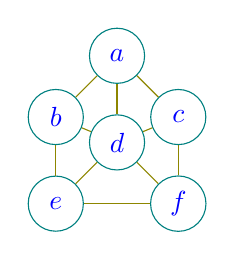
\begin{tikzpicture}[auto,node distance=1.1cm,scale=1, main/.style = {minimum size=0.7cm, color=teal, draw, circle},
                every path/.style = {color=olive}]
                \node[main] (1) {$\bluea$};
                \node[main] (2) [below left of=1] {$\blueb$};
                \node[main] (3) [below right of=1] {$\bluec$};
                \node[main] (4) [below of=1] {$\blued$};
                \node[main] (5) [below of=2] {$\bluee$};
                \node[main] (6) [below of=3] {$\bluef$};
                \path[every node/.style={font=\sffamily\small}]
                    (1) edge node [right] {} (2)
                    (1) edge node [right] {} (3)
                    (1) edge node [right] {} (4)
                    (2) edge node [right] {} (4)
                    (3) edge node [right] {} (4)
                    (2) edge node [right] {} (5)
                    (3) edge node [right] {} (6)
                    (4) edge node [right] {} (5)
                    (4) edge node [right] {} (6)
                    (5) edge node [right] {} (6);
            \end{tikzpicture}

            \pause
            $\n \coloneq |\V| = 6 \geq 3 \jump \vdash \jump \orefirstcond$

            \pause

            \vspace{5px}
            {\footnotesize $\gdeg(\bluea) + \gdeg(\bluee) = 6 \pause \geq \n$
            
            \pause

            $\gdeg(\bluea) + \gdeg(\bluef) = 6 \pause \geq \n$

            \pause

            $\gdeg(\blueb) + \gdeg(\bluec) = 6 \pause \geq \n$
            
            \pause

            $\gdeg(\blueb) + \gdeg(\bluef) = 6 \pause \geq \n$
            
            \pause

            $\gdeg(\bluec) + \gdeg(\bluee) = 6 \pause \geq \n$}

            \pause

            $\vdash \oresecondcond$

            \pause

            \vspace{5px}

            This graph \textbf{satisfies} $\ore$ and \textbf{has}
            
            a Hamiltonian cycle $\T = \textcolor{orange}{\{d,a,b,e,f,c,d\}}.$
        \end{figure}
    \end{frame}

    % This slide is a repeat of the last one but only because it displays the Hamiltonian cycle with arrows.
    \begin{frame}{Example I}
        \begin{figure}
            \emph{First Case}
            
            \small $\Gone(\V,\E)$ \textbf{satisfies} Ore's theorem $\ore$ and \textbf{has} a Hamiltonian cycle $\T$.

            \vspace{5px}
            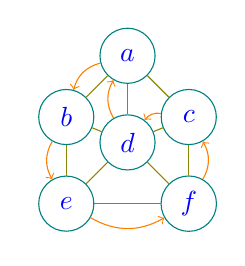
\begin{tikzpicture}[auto,node distance=1.1cm,scale=1, main/.style = {minimum size=0.7cm, color=teal, draw, circle}]
                \node[main] (1) {$\bluea$};
                \node[main] (2) [below left of=1] {$\blueb$};
                \node[main] (3) [below right of=1] {$\bluec$};
                \node[main] (4) [below of=1] {$\blued$};
                \node[main] (5) [below of=2] {$\bluee$};
                \node[main] (6) [below of=3] {$\bluef$};
                \path[every node/.style={font=\sffamily\small},{color=olive}]
                    (1) edge node [right] {} (2)
                    (1) edge node [right] {} (3)
                    (1) edge node [right] {} (4)
                    (2) edge node [right] {} (4)
                    (3) edge node [right] {} (4)
                    (2) edge node [right] {} (5)
                    (3) edge node [right] {} (6)
                    (4) edge node [right] {} (5)
                    (4) edge node [right] {} (6)
                    (5) edge node [right] {} (6);
                \path[->,every node/.style={font=\sffamily\small},{color=orange}]
                    (4) edge[bend left] node [left] {} (1)
                    (1) edge[bend right] node [left] {} (2)
                    (2) edge[bend right] node [left] {} (5)
                    (5) edge[bend right] node [left] {} (6)
                    (6) edge[bend right] node [left] {} (3)
                    (3) edge[bend right] node [left] {} (4);
            \end{tikzpicture}

            $\n \coloneq |\V| = 6 \geq 3 \jump \vdash \jump \orefirstcond$


            \vspace{5px}
            {\footnotesize $\gdeg(\bluea) + \gdeg(\bluee) = 6 \geq \n$

            $\gdeg(\bluea) + \gdeg(\bluef) = 6 \geq \n$

            $\gdeg(\blueb) + \gdeg(\bluec) = 6 \geq \n$

            $\gdeg(\blueb) + \gdeg(\bluef) = 6 \geq \n$

            $\gdeg(\bluec) + \gdeg(\bluee) = 6 \geq \n$}

            $\vdash \oresecondcond$

            \vspace{5px}

            This graph \textbf{satisfies} $\ore$ and \textbf{has}
            
            a Hamiltonian cycle $\T = \textcolor{orange}{\{d,a,b,e,f,c,d\}}.$
        \end{figure}
    \end{frame}

    %% Create a second example of Ore's theorem.
    \begin{frame}{Example II}
        \begin{figure}
            \emph{Second Case}
            
            \small $\Gtwo(\V,\E)$ \textbf{does not satisfy} $\ore$ and \textbf{does not have} a Hamiltonian cycle $\T$.

            \vspace{5px}
            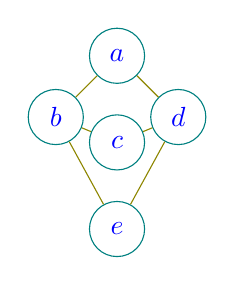
\begin{tikzpicture}[auto,node distance=1.1cm,scale=1, main/.style = {minimum size=0.7cm, color=teal, draw, circle}]
                \node[main] (1) {$\bluea$};
                \node[main] (2) [below left of=1] {$\blueb$};
                \node[main] (3) [below of=1] {$\bluec$};
                \node[main] (4) [below right of=1] {$\blued$};
                \node[main] (5) [below of=3] {$\bluee$};
                \path[every node/.style={font=\sffamily\small},{color=olive}]
                    (1) edge node [right] {} (2)
                    (1) edge node [right] {} (4)
                    (2) edge node [right] {} (3)
                    (3) edge node [right] {} (4)
                    (2) edge node [right] {} (5)
                    (4) edge node [right] {} (5);
            \end{tikzpicture}

            \pause
            $\n \coloneq |\V| = 5 \geq 3 \jump \vdash \jump \orefirstcond$

            \pause

            \vspace{5px}
            {\footnotesize $\gdeg(\bluea) + \gdeg(\bluec) = 4 \pause \ngeq \n$
            
            \pause

            $\gdeg(\bluea) + \gdeg(\bluee) = 4 \ngeq \n$

            $\gdeg(\blueb) + \gdeg(\blued) = 6 \geq \n$

            $\gdeg(\bluec) + \gdeg(\bluee) = 4 \ngeq \n$}

            \pause

            $\cancel\vdash \text{ } \oresecondcond$

            \pause

            \vspace{5px}

            This graph \textbf{does not satisfy} $\ore$ and
            
            \textbf{does not have} a Hamiltonian cycle.
        \end{figure}
    \end{frame}

    %% Create a third example of Ore's theorem.
    \begin{frame}{Example III}
        \begin{figure}
            \emph{Third Case}
            
            \small $\Gthree(\V,\E)$ \textbf{does not satisfy} $\ore$ and \textbf{has} a Hamiltonian cycle $\T$.

            \vspace{5px}
            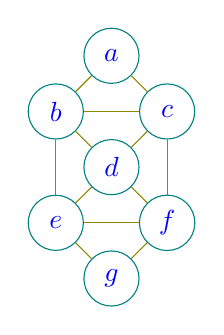
\begin{tikzpicture}[auto,node distance=1cm,scale=1, main/.style = {minimum size=0.7cm, color=teal, draw, circle},
                every path/.style = {color=olive}]
                \node[main] (1) {$\bluea$};
                \node[main] (2) [below left of=1] {$\blueb$};
                \node[main] (3) [below right of=1] {$\bluec$};
                \node[main] (4) [below right of=2] {$\blued$};
                \node[main] (5) [below left of=4] {$\bluee$};
                \node[main] (6) [below right of=4] {$\bluef$};
                \node[main] (7) [below right of=5] {$\blueg$};
                \path[every node/.style={font=\sffamily\small}]
                    (1) edge node [right] {} (2)
                    (1) edge node [right] {} (3)
                    (2) edge node [right] {} (3)
                    (2) edge node [right] {} (4)
                    (2) edge node [right] {} (5)
                    (3) edge node [right] {} (4)
                    (3) edge node [right] {} (6)
                    (4) edge node [right] {} (5)
                    (4) edge node [right] {} (6)
                    (5) edge node [right] {} (6)
                    (5) edge node [right] {} (7)
                    (6) edge node [right] {} (7);
            \end{tikzpicture}

            \pause
            $\n \coloneq |\V| = 7 \geq 3 \jump \vdash \jump \orefirstcond$

            \pause

            \vspace{5px}
            {\scriptsize $\gdeg(\bluea) + \gdeg(\blued) = 6 \ngeq \n$ \quad
            $\gdeg(\bluea) + \gdeg(\bluee) = 8 \geq \n$ \quad
            $\gdeg(\bluea) + \gdeg(\bluef) = 8 \geq \n$

            \pause

            $\gdeg(\bluea) + \gdeg(\blueg) = 4 \ngeq \n $ \quad
            $\gdeg(\blueb) + \gdeg(\bluef) = 8 \geq \n $ \quad
            $\gdeg(\blueb) + \gdeg(\blueg) = 8 \geq \n$
            

            $\gdeg(\bluec) + \gdeg(\bluee) = 8 \geq \n$ \quad
            $\gdeg(\bluec) + \gdeg(\blueg) = 8 \geq \n$ \quad
            $\gdeg(\blued) + \gdeg(\blueg) = 6 \ngeq \n$}

            $\cancel\vdash \text{ } \oresecondcond$

            \pause

            \vspace{5px}

            This graph \textbf{does not satisfy} $\ore$ but still \textbf{has}
            
            a Hamiltonian cycle $\T = \textcolor{orange}{\{a,b,d,e,g,f,c,a\}}$.
        \end{figure}
    \end{frame}

    % This slide is a repeat of the last one but only because it displays the Hamiltonian cycle with arrows.
    \begin{frame}{Example III}
        \begin{figure}
            \emph{Third Case}
            
            \small $\Gthree(\V,\E)$ \textbf{does not satisfy} $\ore$ and \textbf{has} a Hamiltonian cycle $\T$.

            \vspace{5px}
            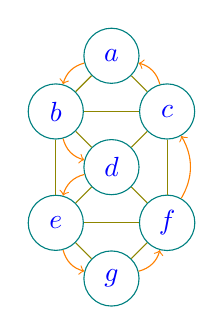
\begin{tikzpicture}[auto,node distance=1cm,scale=1, main/.style = {minimum size=0.7cm, color=teal, draw, circle}]
                \node[main] (1) {$\bluea$};
                \node[main] (2) [below left of=1] {$\blueb$};
                \node[main] (3) [below right of=1] {$\bluec$};
                \node[main] (4) [below right of=2] {$\blued$};
                \node[main] (5) [below left of=4] {$\bluee$};
                \node[main] (6) [below right of=4] {$\bluef$};
                \node[main] (7) [below right of=5] {$\blueg$};
                \path[every node/.style={font=\sffamily\small},{color=olive}]
                    (1) edge node [right] {} (2)
                    (1) edge node [right] {} (3)
                    (2) edge node [right] {} (3)
                    (2) edge node [right] {} (4)
                    (2) edge node [right] {} (5)
                    (3) edge node [right] {} (4)
                    (3) edge node [right] {} (6)
                    (4) edge node [right] {} (5)
                    (4) edge node [right] {} (6)
                    (5) edge node [right] {} (6)
                    (5) edge node [right] {} (7)
                    (6) edge node [right] {} (7);
                \path[->,every node/.style={font=\sffamily\small},{color=orange}]
                    (1) edge[bend right] node [left] {} (2)
                    (2) edge[bend right] node [left] {} (4)
                    (4) edge[bend right] node [left] {} (5)
                    (5) edge[bend right] node [left] {} (7)
                    (7) edge[bend right] node [left] {} (6)
                    (6) edge[bend right] node [left] {} (3)
                    (3) edge[bend right] node [left] {} (1);
            \end{tikzpicture}

            $\n \coloneq |\V| = 7 \geq 3 \jump \vdash \jump \orefirstcond$

            \vspace{5px}
            {\scriptsize $\gdeg(\bluea) + \gdeg(\blued) = 6 \ngeq \n$ \quad
            $\gdeg(\bluea) + \gdeg(\bluee) = 8 \geq \n$ \quad
            $\gdeg(\bluea) + \gdeg(\bluef) = 8 \geq \n$

            $\gdeg(\bluea) + \gdeg(\blueg) = 4 \ngeq \n $ \quad
            $\gdeg(\blueb) + \gdeg(\bluef) = 8 \geq \n $ \quad
            $\gdeg(\blueb) + \gdeg(\blueg) = 8 \geq \n$
            

            $\gdeg(\bluec) + \gdeg(\bluee) = 8 \geq \n$ \quad
            $\gdeg(\bluec) + \gdeg(\blueg) = 8 \geq \n$ \quad
            $\gdeg(\blued) + \gdeg(\blueg) = 6 \ngeq \n$}

            $\cancel\vdash \text{ } \oresecondcond$

            \vspace{5px}

            This graph \textbf{does not satisfy} $\ore$ but still \textbf{has}
            
            a Hamiltonian cycle $\T = \textcolor{orange}{\{a,b,d,e,g,f,c,a\}}$.
        \end{figure}
    \end{frame}

  %% Describe the applications of graph theory and relate that to Hamiltonian
    %% paths and the importance of efficiency in finding them. This can be as
    %% many slides as you want.

    \begin{frame}{Applications}
   
        \textbf{Hamiltonian cycles} have a variety of real-world applications.

        \vspace{10px}

        \textcolor{blue}{Network routing:}
        \begin{itemize}
            \item finding the most effective and efficient round-trip path between points A to B
            \item improving network traffic by reducing delays from client to server
            \item optimizing network runtime
        \end{itemize}

        \vspace{20px}

        Picture a data packet moving through a network of routers to reach a server, aiming to find a path that visits each router exactly once, and thereby optimizing data transmission efficiency.

    \end{frame}

    \begin{frame}{Applications}
        \textbf{Hamiltonian cycles} have a variety of real-world applications.

        \vspace{10px}

        \textcolor{blue}{Navigation systems:}
        \begin{itemize}
            \item finding a path that travelers can take to both reach every destination and reduce estimated time of arrival
            \item development of algorithms to prevent travelers from revisiting destinations and inefficient paths
        \end{itemize}
        
        \vspace{20px}

        In some navigation systems, the primary goal is to find an efficient \emph{round-trip} cycle that visits each destination once, ensuring smooth transport without revisiting locations.

        % for this example while in the video, I will explain more in detail.
        % Essentially is the idea of how a certain case, navigation technology
        % re computes and performs a new hamiltonian path that is efficient for
        % the driver/traveler to avoid traffic and travel time
        % - Gabriel Serrano

        % That is fine. I edited this section as an example is better spoken as
        % opposed to put in the slide. Extra space was used to provide more abstract
        % examples. If you'd like the example you gave so you can give yourself somewhat
        % of a script, here it is: "Traffic in the US 60W freeway to Los Angeles"
        % - Youssef Adam

    \end{frame}

    %% Summarize everything this presentation has covered, from the statement of Ore's Theorem to its Applications.
    \begin{frame}{Conclusion: Summary}
        Ore's theorem has many practical, mathematical applications.
        
        This theorem can be applied to anything that deals with systems that can be represented
        by vertices and graph, such as:
        \begin{multicols}{2}
            \begin{itemize}
            \item transportation systems
            \item neural networks
            \item sewage pipes
            \end{itemize}
            
            \columnbreak

            \begin{itemize}
            \item electrical lines
            \item social networks
            \end{itemize}
            \end{multicols}
            Any individual can apply this theorem to solve problems
            involving such matters. Ore's theorem is a revolutionary theorem that has
            enabled humanity to progress expeditiously in the field of mathematics and
            technological innovations.
    \end{frame}

    %% Restate the questions.
    \begin{frame}{Conclusion: Questions}
        Below are the questions displayed at the beginning of the presentation.
        \vspace{10px}
        \begin{itemize}
            \item What are the two criteria a graph must meet in order to satisfy Ore's theorem and therefore be a Hamiltonian graph?
            \item If a graph $\G$ does not meet both criteria to satisfy Ore's theorem, is $\G$ Hamiltonian?
            \item What is one example of a real-world application of Hamiltonian cycles, and how does this tie in with Ore's theorem?
        \end{itemize}
    \end{frame}

\end{document}
